\documentclass[a4paper, 11pt]{article}
\usepackage[utf8]{inputenc}
\usepackage[czech]{babel}
\usepackage[total={18.5cm, 25cm}, top=1cm, bottom=1cm, left=1.25cm, includehead]{geometry}
\usepackage{fancyhdr} %záhlaví
\usepackage{amsmath} % větší zlomyk pmocí \dfrac
\usepackage{fixmath} % bolt matika pomocí \mathbold
\usepackage{tikz}% balík využívaný circuitikz
\usepackage[european, american inductors]{circuitikz} % elektrická schémata
\usepackage{siunitx} % SI jednotky
\usepackage{graphicx}
\usepackage{float} % H aby neuplavali
\usepackage{tabularx} % tabulka s možností X
\usepackage{ctable} % horozontální čára s nastavitelnou šířkou a mezerami od okolí \specialrule{1pt}{0pt}{0pt}

\usepackage{pdflscape} % stránka na šířku
\usepackage{pdfpages} % vložení pdf stránky

\usepackage{hyperref}
\hypersetup{
    colorlinks=true,
    linkcolor=blue,
    filecolor=magenta,
    urlcolor=cyan,
}

\urlstyle{same}

\usepackage{array}
\usepackage{multirow} % více řádků

\usepackage[formats]{listings} % Balíček pro sazbu zdrojových textů

\usepackage{color}

\definecolor{codegreen}{rgb}{0,0.6,0}
\definecolor{codegray}{rgb}{0.5,0.5,0.5}
\definecolor{codepurple}{rgb}{0.58,0,0.82}
\definecolor{backcolour}{rgb}{0.95,0.95,0.92}

\lstdefinestyle{mystyle}{
    backgroundcolor=\color{backcolour},
    commentstyle=\color{codegreen},
    keywordstyle=\color{magenta},
    numberstyle=\tiny\color{codegray},
    stringstyle=\color{codepurple},
    basicstyle=\footnotesize,
    breakatwhitespace=false,
    breaklines=true,
    captionpos=b,
    keepspaces=true,
    numbers=left,
    numbersep=5pt,
    showspaces=false,
    showstringspaces=false,
    showtabs=false,
    tabsize=2
}

\lstset{style=mystyle}

\lstset{
language=C++,                	  % choose the language of the code
numbers=left,                   % where to put the line-numbers
stepnumber=1,                   % the step between two line-numbers.
numbersep=5pt,                  % how far the line-numbers are from the code
backgroundcolor=\color{backcolour},  % choose the background color. You must add \usepackage{color}
showspaces=false,               % show spaces adding particular underscores
showstringspaces=false,         % underline spaces within strings
showtabs=false,                 % show tabs within strings adding particular underscores
tabsize=2,                      % sets default tabsize to 2 spaces
captionpos=b,                   % sets the caption-position to bottom
breaklines=true,                % sets automatic line breaking
breakatwhitespace=true,         % sets if automatic breaks should only happen at whitespace
%title=~%firmware kostky 08.12.2016,                 % show the filename of files included with \lstinputlisting;
%    Definice jazyka použitého ve výpisech
%    language=[LaTeX]{TeX},    % LaTeX
%    language={Matlab},        % Matlab
    inputencoding=utf8,        % pro soubory uložené v kódování UTF-8
    %inputencoding=cp1250,     % pro soubory uložené ve standardním kódování Windows CP1250
%        columns=fixed,         %flexible,
%        fontadjust=true        %licovani sloupcu
    extendedchars=true,
    literate=                  % definice symbolů s diakritikou
    {á}{{\'a}}1
    {č}{{\v{c}}}1
    {ď}{{\v{d}}}1
    {é}{{\'e}}1
    {ě}{{\v{e}}}1
    {í}{{\'i}}1
    {ň}{{\v{n}}}1
    {ó}{{\'o}}1
    {ř}{{\v{r}}}1
    {š}{{\v{s}}}1
    {ť}{{\v{t}}}1
    {ú}{{\'u}}1
    {ů}{{\r{u}}}1
    {ý}{{\'y}}1
    {ž}{{\v{z}}}1
    {Á}{{\'A}}1
    {Č}{{\v{C}}}1
    {Ď}{{\v{D}}}1
    {É}{{\'E}}1
    {Ě}{{\v{E}}}1
    {Í}{{\'I}}1
    {Ň}{{\v{N}}}1
    {Ó}{{\'O}}1
    {Ř}{{\v{R}}}1
    {Š}{{\v{S}}}1
    {Ť}{{\v{T}}}1
    {Ú}{{\'U}}1
    {Ů}{{\r{U}}}1
    {Ý}{{\'Y}}1
    {Ž}{{\v{Z}}}1
}


\usepackage{pdfpages}

% moje vlastní příkazy ===========================
\newcommand{\predmet}{Implementace Komunikačních Systémů}
\newcommand{\uloha}{\textsc{Demodulace frekvenčního klíčování FSK}}
\newcommand{\rocnik}{1}
\newcommand{\autor}{\textsc{Jan Vykydal} \\ ID: 186240}

\newcommand{\vcara}{{\vrule width 1pt}}
\newcommand{\hcara}{\specialrule{1pt}{0pt}{0pt}}
\newcommand*{\thead}[1]{\multicolumn{1}{c}{\bfseries #1}}
% konec mích vlastních příkazů ===================


\pagestyle{fancy}
\fancyhf{}
% jednostranná sazba
\fancyhead[L]{
    \begin{tabular}{lr}
        \textsc{Jan Vykydal} \\
        186240
    \end{tabular}
}
\fancyhead[C]{
    \begin{tabular}{c}
        \textsc{\predmet} \\
        \textsc{\uloha}
    \end{tabular}
}
\fancyhead[R]{
    \begin{tabular}{lr}
        \multicolumn{2}{r}{FEKT UREL} \\
        \textsc{List:} & \thepage/\pageref{konec}
    \end{tabular}
}
%\fancyfoot[C]{\textbf{List:} \thepage/\pageref{konec}}

\renewcommand{\headrulewidth}{0.4pt}
%\renewcommand{\footrulewidth}{0.4pt}



\begin{document}
    %\renewcommand{\figurename}{Schéma č.}
    \renewcommand{\tablename}{Tabulka č.}
    \setcounter{page}{1}

    \section*{Úvod}

FSK modulace je založená na technice frekvenčního klíčování. Funguje to tak, že jednotlivým vysílaným symbolům (0, 1) odpovídá harmonický signál o definované frekvenci.

Realizovaný systém si klade za cíl demodulovat a posléze dekódovat správy vysílané modemem BEL202. Úrovni logické jedničky odpovídá kmitočet $1,2~kHz$ a logické nule $2,2~kHz$.

\begin{figure}[H]
    \centering
    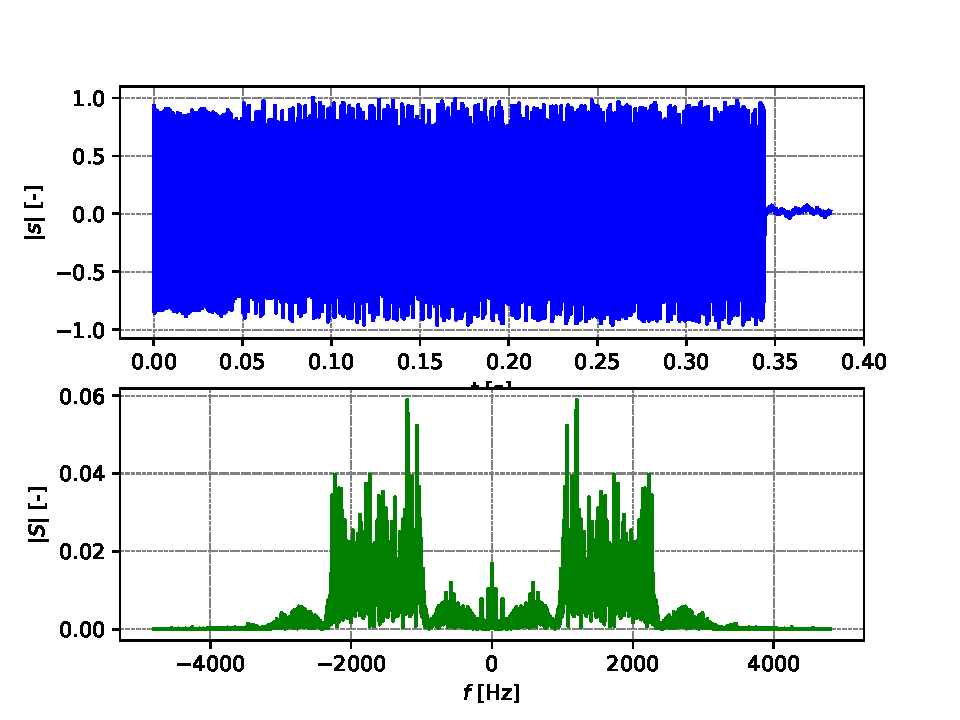
\includegraphics[width=\textwidth]{img/wav.pdf}
    \caption{Časový průběh a frekvenční modulové spektrum vstupního souboru \texttt{1.wav}}
\end{figure}

Jak je ve spektru vidět, nejvíce jsou zastoupeny kmitočty okolo $1,2~kHz$ a $2,2~kHz$, zároveň je v signálu i značné množství šumu.
    \clearpage

\section*{Přizpůsobený filtr}

\begin{figure}[H]
    \centering
    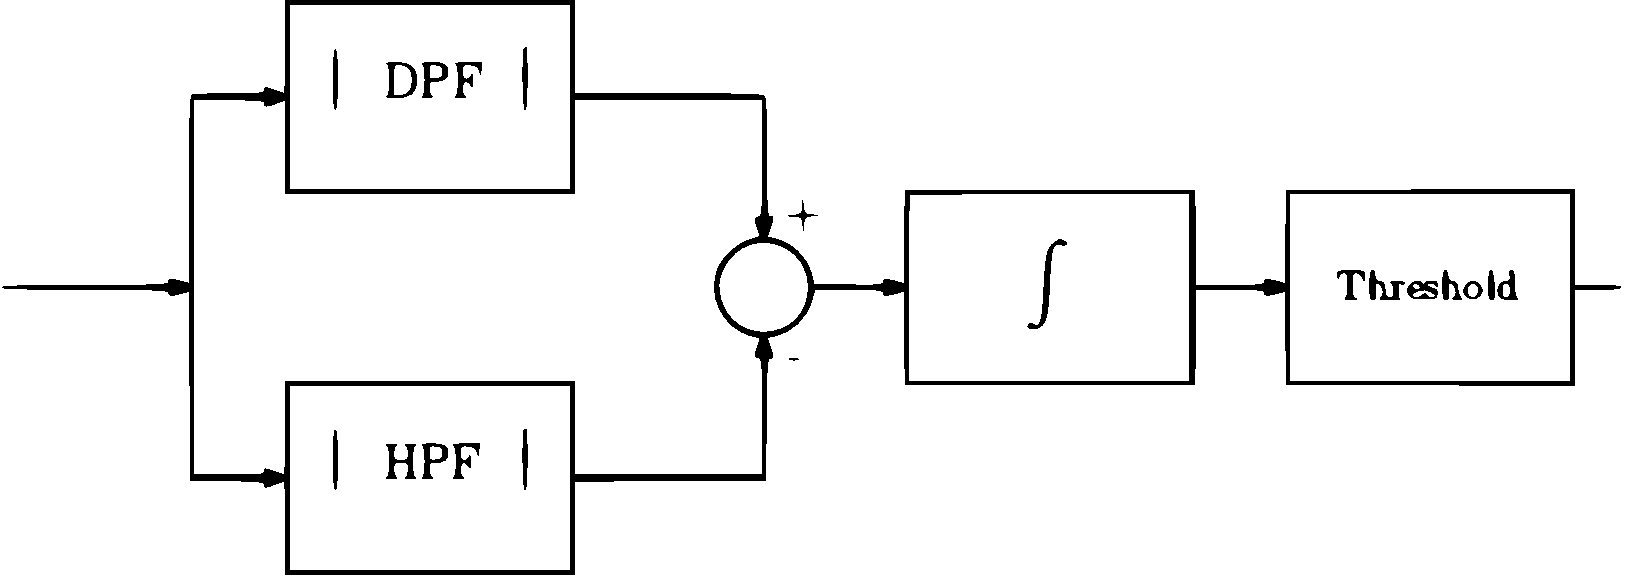
\includegraphics[width=0.5\textwidth]{img/dem1.pdf}
    \caption{Blokové schéma demodulátoru s přizpůsobeným filtrem}
\end{figure}

Tato metoda bude dále označována jako DEM1. Nejprve dojde k rozdělení signálu pomocí horní a dolní propusti. Následně je spočítána absolutní hodnota z filtrovaných signálů, což představuje usměrnění. Díky tomu je možné signály od sebe odečíst. Tím vznikne signál ve kterém vyšším hodnotám odpovídá 1 nízkým 0. Poté signál integrujeme podle času, tedy opět na něj aplikujeme dolní propust. Nyní je signál již připraven k prahování, pomocí kterého rozhodneme zda-li je přijímána logická nula nebo jednička.

\begin{figure}[H]
    \centering
    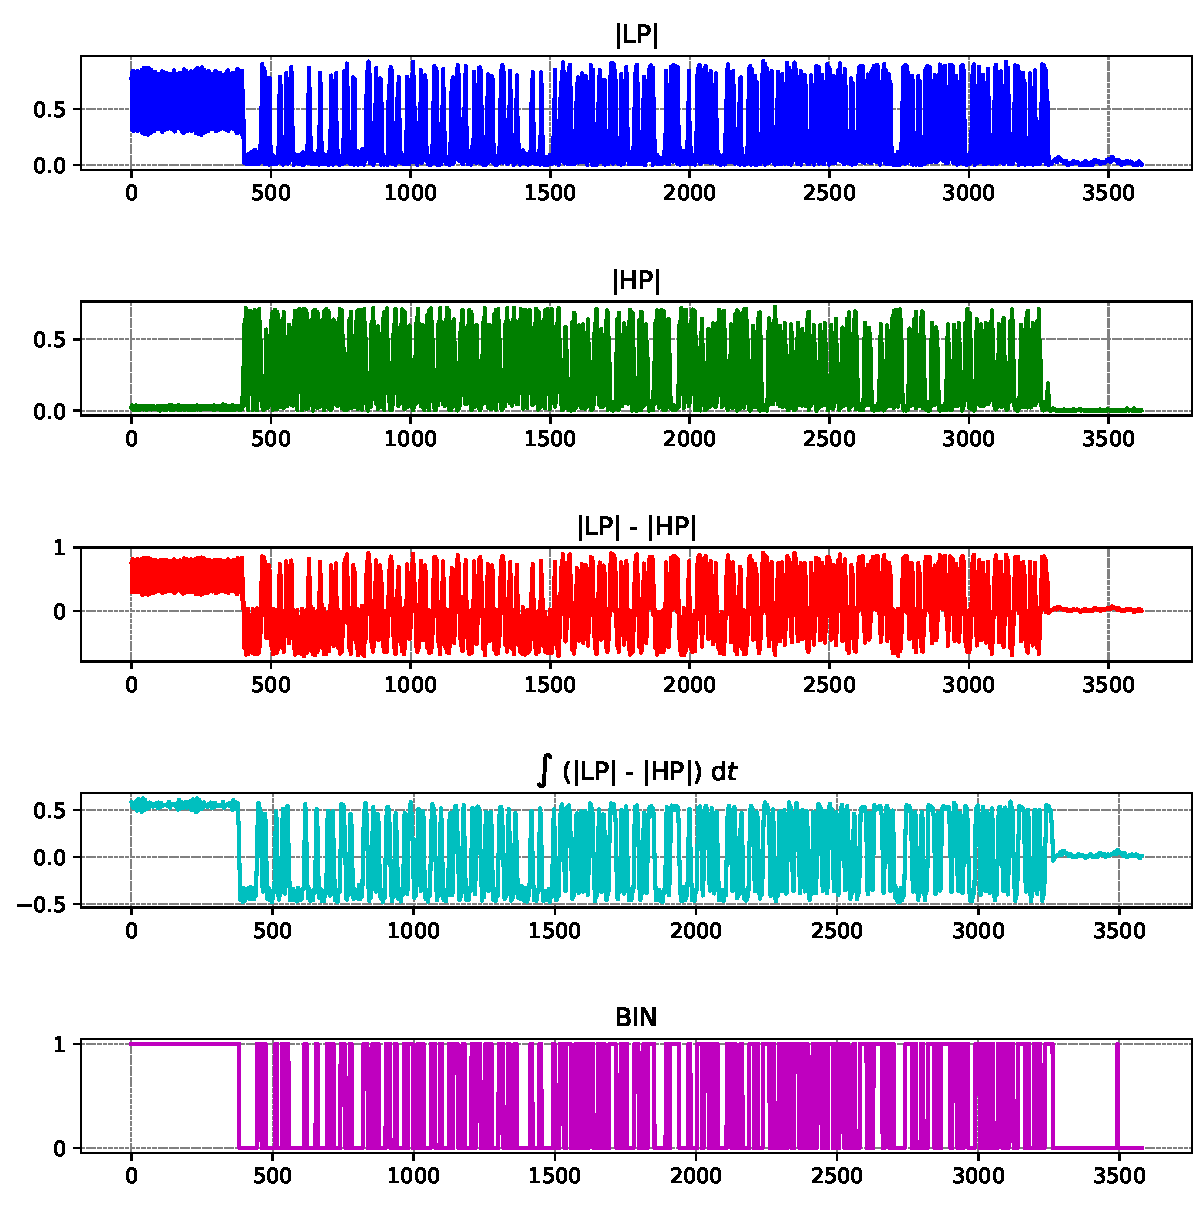
\includegraphics[width=0.85\textwidth]{img/dem1_graph.pdf}
    \caption{Časové průběhy bloků demodulátoru}
\end{figure}
    \section*{Korelační přijímač}

Korelační přijímač dále DEM2 provádí korelaci vstupního signálu s bázovými signály, ty odpovídají harmonickým signálům $1,2~kHz$ a $2,2~kHz$. Navíc pro každý z kmitočtů jsou vytvořeny rovnou dva bázové signály posunuté o $\frac{\pi}{2}$. To je kvůli tomu aby korelace měla dostatečnou hodnotu pro libovolnou počáteční fázi. Kvadráty odpovídajících korelací jsou dále sečteny a filtrovány dolní propustí. Tímto postupem získám dva signály det$_1$ a det$_2$, ty jsou nakonec porovnány, čím získáme binární signál.

\begin{figure}[H]
    \centering
    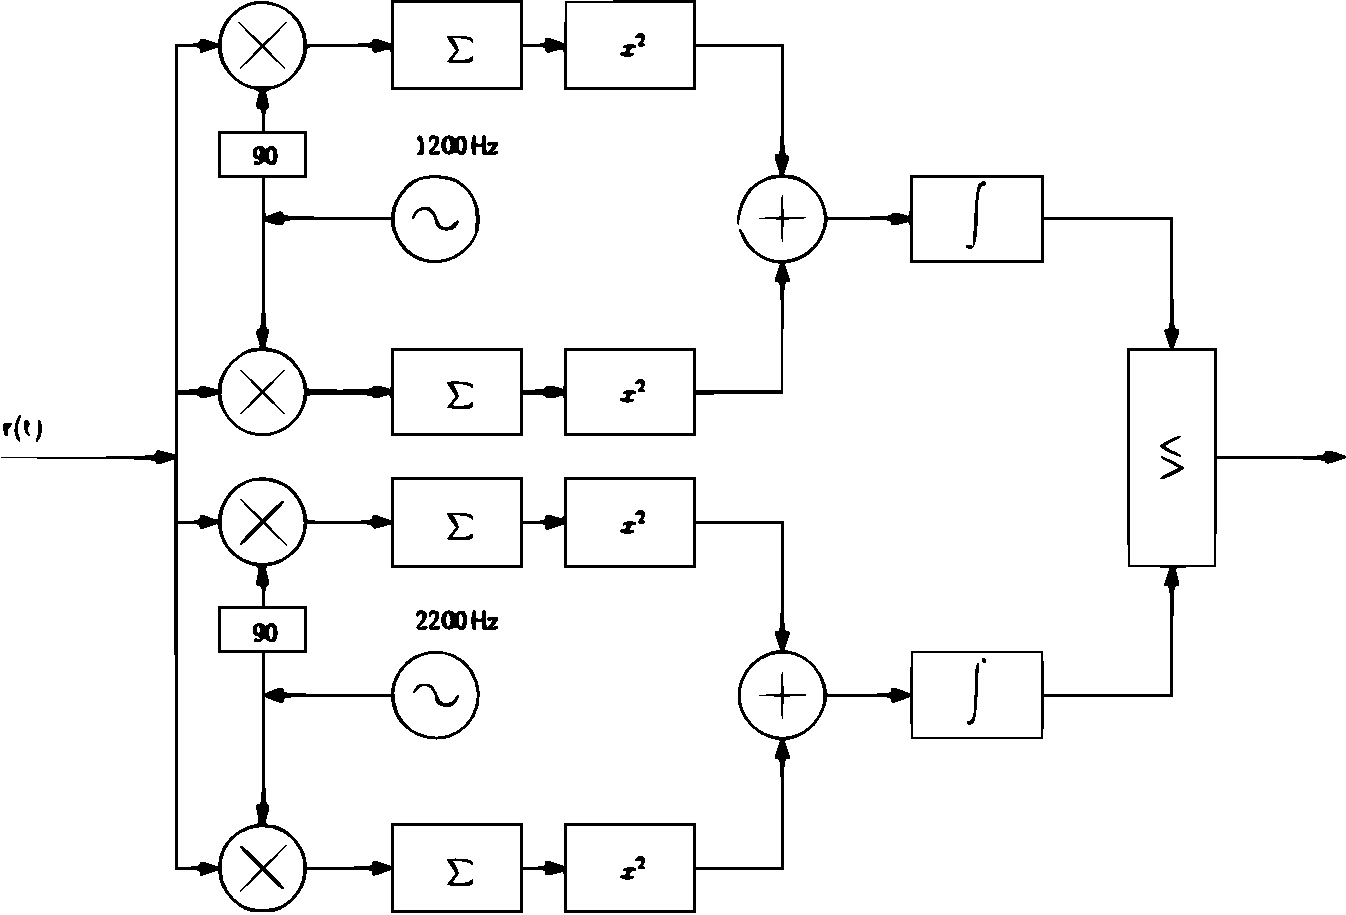
\includegraphics[width=\textwidth]{img/dem2.pdf}
    \caption{Blokové schéma demodulátoru s korelátorem}
\end{figure}

\begin{figure}[H]
    \centering
    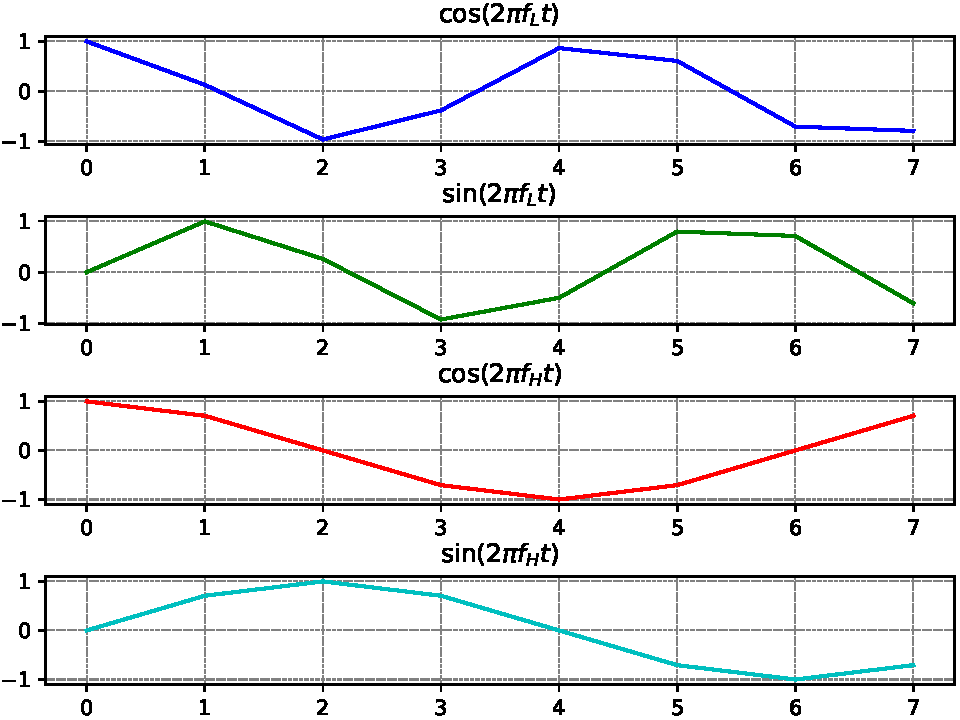
\includegraphics[width=0.8\textwidth]{img/base.pdf}
    \caption{Bázové funkce pro korelátor}
\end{figure}

\begin{figure}[H]
    \centering
    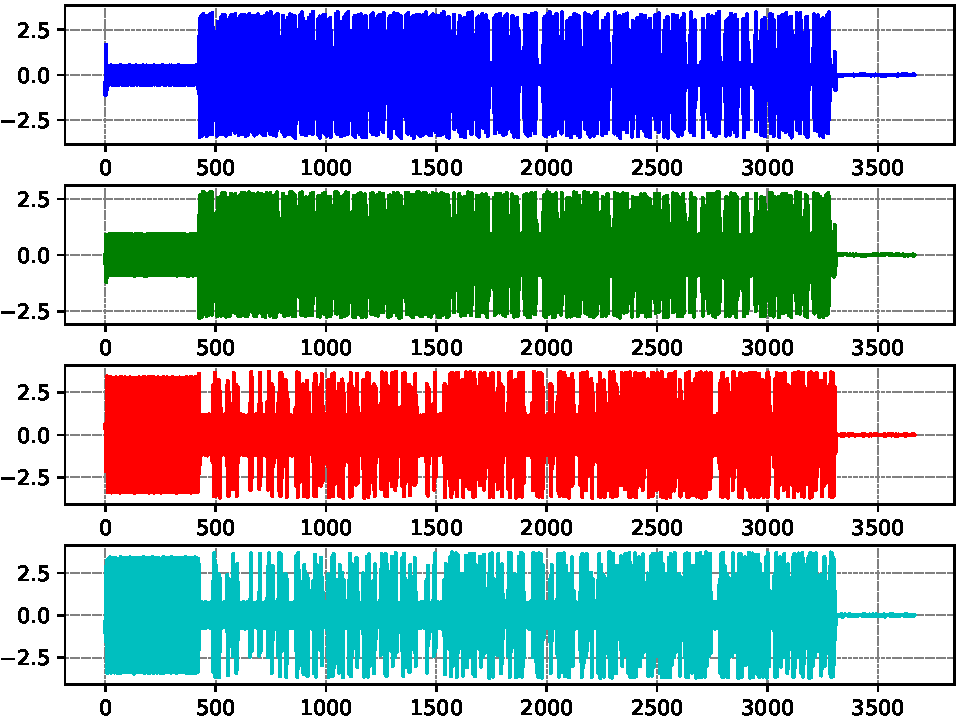
\includegraphics[width=0.8\textwidth]{img/cor.pdf}
    \caption{Korelace vstupního signálu s bázovými funkcemi, barvy odpovídají bázovým funkcím}
\end{figure}

\begin{figure}[H]
    \centering
    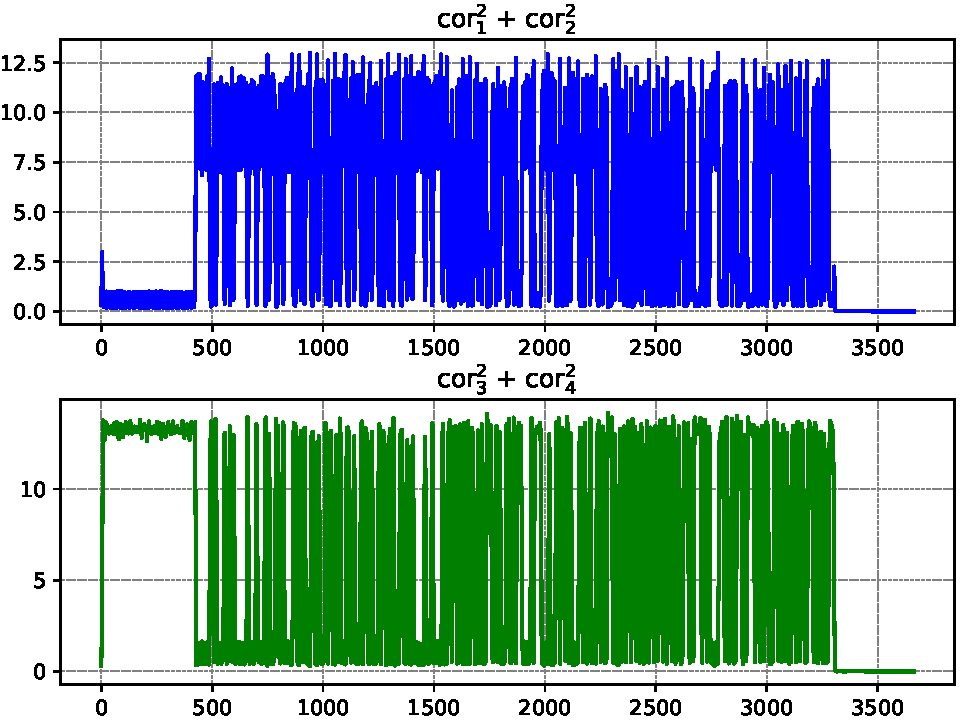
\includegraphics[width=0.7\textwidth]{img/cor_sum.pdf}
    \caption{Součty kvadrátů odpovídajících bázových funkcí ($\sin$ a $\cos$ stejné frekvence)}
\end{figure}

\begin{figure}[H]
    \centering
    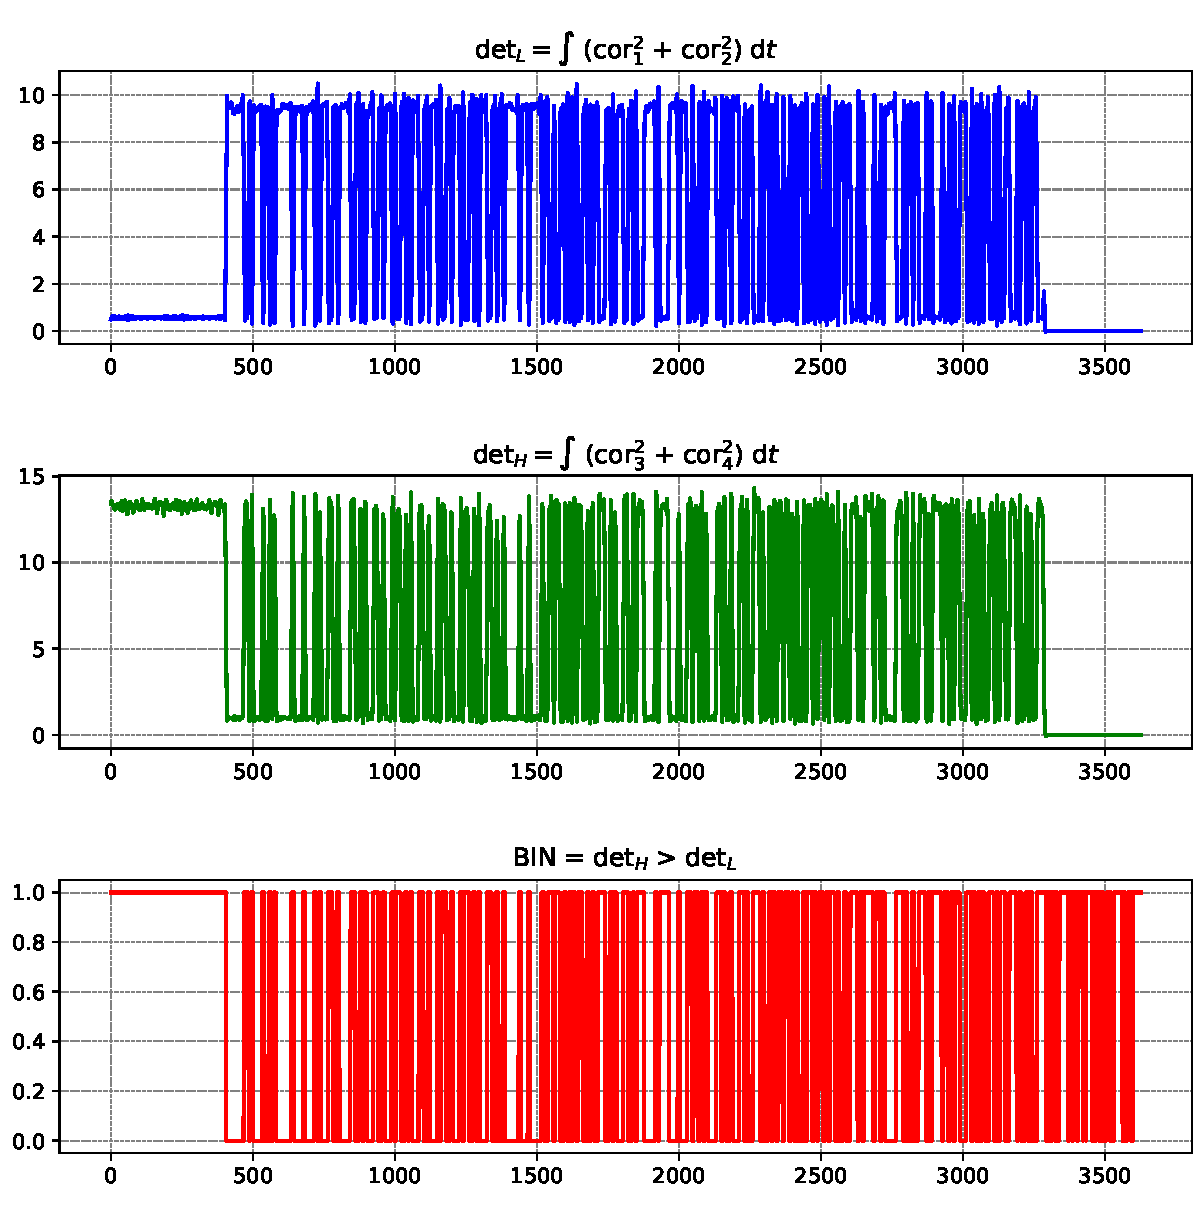
\includegraphics[width=0.7\textwidth]{img/dem2_graph.pdf}
    \caption{Časové průběhy výstupů detektoru a získaného binárního signálu}
\end{figure}
    \section*{Závěr}

Oby dva demodulátory jsem podrobil testu spočívajícího v zašumění vstupního signálu. Hodnoty odstupu signálu od šumu SNR $\in \langle 2; 14 \rangle~dB$. SNR bylo krokováno po $0,05~dB$ a na každou úroveň SNR proběhlo 100~000 demodulačních cyklů.

\begin{figure}[H]
    \centering
    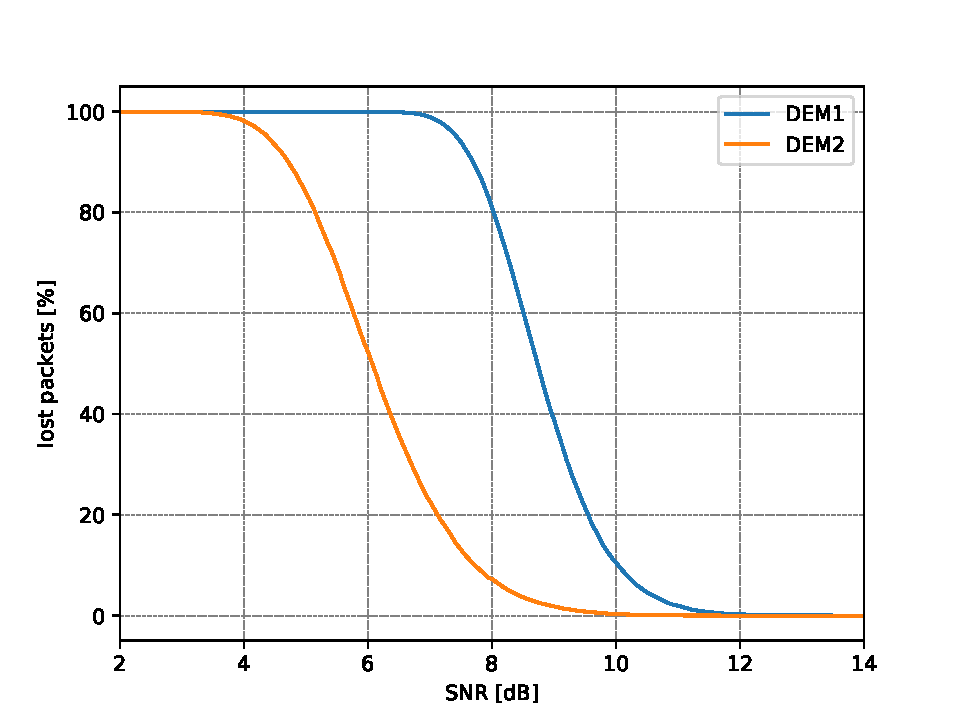
\includegraphics[width=\textwidth]{img/lost_packets.pdf}
    \caption{Závislost chybovosti na SNR}
\end{figure}


\begin{enumerate}
    \item  Z provedeného experimentu lze pozorovat, že DEM1 dosáhne nulové chybovosti při SNR$ = 12~dB$ a DEM2 při SNR$ = 10~dB$. DEM2 je tedy schopen  demodulovat více zašumělý signál.
    \item DEM1 je velmi citlivý na hodnotu prahu, nejlepších výsledků jsem dosáhl s prahem 0,7.
    \item Dalším parametrem který má velký vliv na obě metody demodulátoru jsou filtry. Čím mají filtry větší rozdíl útlumu mezi propustným a nepropustným pásmem tím jsou vhodnější. Také je důležité správně zvolit mezní frekvence filtrů.
\end{enumerate}

\begin{figure}[H]
    \centering
    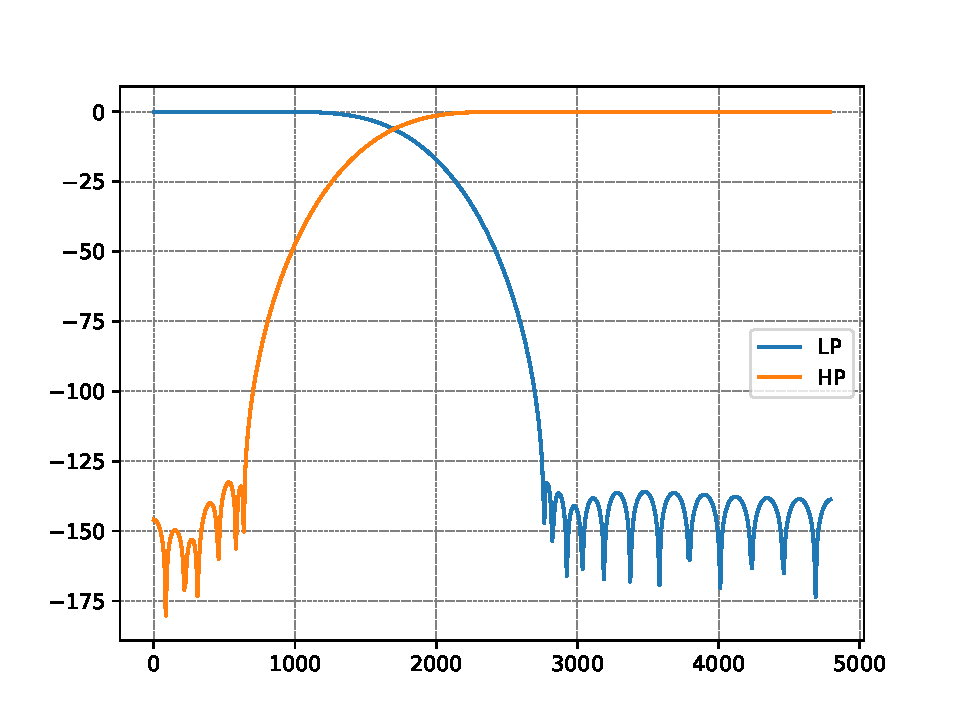
\includegraphics[width=0.8\textwidth]{img/filter.pdf}
    \caption{Frekvenční charakteristiky navržených filtrů}
\end{figure}

Jedná se o FIR filtry, tedy filtry s konečnou impulzní odezvou. Navrženy jsou pomocí metody okna realizované funkcí \texttt{scipy.signal.firwin}, která vrací impulzní odezvu. Délka impulzní odezvy je 41 vzorků. Použité okno je Kaiserovo s parametrem $\beta = 14$.

\begin{lstlisting}[caption={Dekódování zprávy ze souboru \texttt{1.wav}}]
    80 21 01 08 31 30 31 34 | .!..1014
    31 34 34 31 02 04 36 35 | 1441..65
    39 31 07 0F 6C 61 62 2E | 91..lab.
    6D 69 6B 72 6F 70 72 6F | mikropro
    63 65 73 CA F6 FF E6    | ces....

    Packet length 36 octets
    P1 datetime(MM/DD HH:MM): 10/14 14:41
    P2 caller number: 6591
    P7 caller name: lab.mikroproces
\end{lstlisting}

\begin{lstlisting}[caption={Dekódování zprávy ze souboru \texttt{3.wav}}]
    80 1D 01 08 31 30 31 34 | ....1014
    31 34 35 30 02 04 36 35 | 1450..65
    39 35 07 0B 6C 61 62 2E | 95..lab.
    50 43 36 2E 36 30 61 BE | PC6.60a.
    BD DD                   | ..

    Packet length 32 octets
    P1 datetime(MM/DD HH:MM): 10/14 14:50
    P2 caller number: 6595
    P7 caller name:
                    lab.PC6.60a
\end{lstlisting}

Celý demodulátor je napsaný v Pythonu a dostupný na \url{https://github.com/wykys/MIKS-FSK}. Navíc simulace využívá paralelizaci výpočtů na více jader, takže výpočet probíhá relativně rychle.
    \label{konec}
\end{document}
